\section{Posets of graph rewriting events}

\subsection{From transition systems to posets}
\label{sec:concret}

\begin{definition}[Causal trace]
  \label{def:causal_trace}
  Let $\theta:M_0\overset{m_1,p_1}{\Rightarrow} M_1\overset{m_2,p_2}{\Rightarrow} M_2 \cdots \overset{m_n,p_n}{\Rightarrow} M_n$ be a trace.
  Two transitions $t_1$ and $t_2$ of $\theta$ are low res dependent in $\theta$, if $t_1\prec_{\theta} t_2$ can be derived by the following rules:
  \begin{align*}
    \frac{t_1 \prec t_2}{t_1 \prec_{\theta} t_2}\quad
    \frac{t_1\simeq t_1'\prec t_2'\simeq t_2}{t_1 \prec_{\theta} t_2}
  \end{align*}
  %Two transitions $t_1$ and $t_2$ of $\theta$ are low res dependent in $\theta$, if $t_1\prec_{\theta} t_2$ can be derived by similar rules to the ones above.
  In a similar manner, we define when a transition $t_1$ inhibits a transition $t_2$ of $\theta$, denoted $t_1\dashv_{\theta} t_2$.
  Define $\leq$ the transitive and reflexive closure of low res dependence. We say that $\theta$ is a \emph{causal trace} if it is directed w.r.t. $\leq$.
\end{definition}

\begin{lemma}
  \label{lem:inhibiting_pair}
  Let $t_1$ and $t_2$ be two transitions in a causal trace $\theta$.
  \begin{enumerate}
  \item If $t_1\dashv t_2$ then $t_2\not\dashv t_1$.
  \item If $t_1\leq t_2$ then $t_2\not\dashv t_1$.
  \end{enumerate}
\end{lemma}

\begin{definition}[The abstraction on a trace]
  \label{def:abstraction}
  Let us denote with $\Theta$ the set of causal traces.
  Define $\alpha:\Theta\to\mathcal{S}$ an \emph{abstraction} function that maps a trace into a poset as follows:
  \begin{itemize}
  \item given a transition $t_i:M_i\overset{m,p}{\Rightarrow} M_{i+1}$ define the \emph{abstract event} $\alpha(t_i) = e_i$ such that $\labl(e_i) = p$.
  \item define an augmented poset from a trace $\alpha(\theta) = (E,\prec,\dashv,\labl)$ such that $\alpha$ is a bijection between transitions and abstract events and such that the low res dependence and inhibition relations between transitions is preserved:
    \begin{align*}
      %e_i \cover e_j \iff t_i <_{\theta} t_j \text{ and } \alpha(t_i)=e_i, \alpha(t_j)=e_j\\
      e_i \prec e_j \iff t_i \prec_{\theta} t_j \text{ and } \alpha(t_i)=e_i, \alpha(t_j)=e_j\\
      e_i \dashv e_j \iff t_i \dashv_{\theta} t_j \text{ and } \alpha(t_i)=e_i, \alpha(t_j)=e_j.
    \end{align*}
  \end{itemize}
  Let $\Theta = \{\theta_1,\cdots,\theta_n\}$ be a set of causal traces.
  Define the set of augmented posets $\mathcal{S}$ obtained by abstraction on $\Theta$ as follows
  \[
  \alpha(\{\theta_1,\cdots,\theta_n\}) = (s_1,\cdots, s_k)/_{\iso}\text{ with }k\leq n.
  \]
  %where for each augmented poset $s$ there exists at least one trace $\theta\in\Theta$ such that $\alpha(\theta) = s$.
\end{definition}

\begin{example}
  Let us consider the following rules and trace:
  \begin{align*}
    r_1:A \Rightarrow A, B\qquad r_2:A \Rightarrow C \qquad r_3: B,C \Rightarrow C\qquad
    A \overset{\id_A,r_1}{\Rightarrow} A, B \overset{\id_A,r_2}{\Rightarrow} B,C \overset{id_{B,C},r_3}{\Rightarrow}C.
  \end{align*}
  Let us denote $t_1$, $t_2$ and $t_3$ the three transitions. We have that $t_1\prec t_3$, $t_2\prec t_3$ and $t_2\dashv t_1$.
  Note that if the abstraction also "forgets" that $t_2\dashv t_1$ the concretisation retrieves the trace above and a second one where $t_1$ and $t_2$ are sequential independent:
  \begin{align*}
    A_1,A_2 \overset{\id_{A_1},r_1}{\Rightarrow} A_1,A_2,B \overset{\id_{A_2},r_2}{\Rightarrow} A_1,B,C \overset{id_{B,C},r_3}{\Rightarrow} A_1,C.
  \end{align*}
\end{example}

\subsection{Decorated posets}

\begin{definition}[Decorated poset]
  \label{def:decorate_poset}
  \begin{enumerate}
  \item[] $~$
  \item Given a set of events $E$ and a labeling function $\labl$ on events, define a function $\decor:E\times E \to E\times E\times \spa$ that associates to a pair of events $(e,e')$ the following set
    \begin{align*}
      \decor_{+}(e,e') = \{(e,e',\spa) : \spa\text{ is a span such that }\labl(e)\redl{+}_{\spa} \labl(e')\}\\
       \decor_{-}(e,e') = \{(e,e',\spa) : \spa\text{ is a graph such that }\labl(e)\redl{-}_{\spa} \labl(e')\}
    \end{align*}

  \item Let $s = (E,\prec,\dashv,\labl)$ be an augmented poset. A \emph{decorated} poset of $s$, denoted $s^{\star}$, is defined as follows
    \begin{align*}
      s^{\star} = (E,\redl{+},\redl{-},\labl), \text{ where }
      &e\redl{+}_{\spa} e' \iff (e,e',{\spa})\in\decor_+(e,e')\text{ and }e\prec e'\\
      &e\redl{-}_{\spa} e' \iff (e,e',{\spa})\in\decor_-(e,e')\text{ and }e\dashv e'\\
    \end{align*}
    We denote $\decor(s)$ the set of all decorated posets of $s$.
  \end{enumerate}
\end{definition}

Note that the notation $e\redl{+}_{\spa} e'$ is an overload of the notation $\labl(e)\redl{+}_{\spa} \labl(e')$. The first is \emph{defined} on events while the second holds on rules and can be \emph{inferred} from the rules itselves.

\begin{definition}
  Let $e_1$,$e_2$ be two events in a decorated poset and let $\spa:L_1\remb O\lemb L_2$ be a span. We say that $e_1$ and $e_2$ are \emph{pairs for positive influence w.r.t. $\spa$} if for all events $e_3$ such that $e_3\redl{+}_{\spa_1} e_1$ and $\spa_1:R_3\remb O_1\lemb L_1$ for which the diagram commutes
  \[
  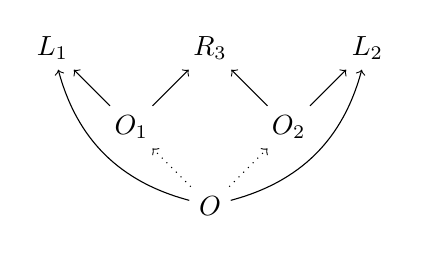
\begin{tikzpicture} %[scale=0.8]
      \node (o) at (0,-1) {\(O\)};
      \node (r3) at (0,1) {\(R_3\)};
      \node (o1) at (-1,0) {\(O_1\)};
      \node (o2) at (1,0) {\(O_2\)};
      \node (r1) at (-2,1) {\(L_1\)};
      \node (r2) at (2,1) {\(L_2\)};
      \draw [dotted,->] (o) -- (o1);
      \draw [dotted,->] (o) -- (o2);
      \draw [->] (o1) -- (r3);
      \draw [->] (o2) -- (r3);
      \draw [->] (o1) -- (r1);
      \draw [->] (o2) -- (r2);
      \draw [->] (o) to [bend left] (r1);
      \draw [->] (o) to [bend right] (r2);
    \end{tikzpicture}
    \]
there exists $\spa_2:R_3\remb O_2\lemb L_2$ that commutes and such that $e_3\redl{+}_{\spa_2} e_2$.
Similarly we say that $e_1$ and $e_2$ are \emph{pairs for negative influence w.r.t. $\spa$} if for any event $e_3$ that has a negative influence on $e_1$ involving some part of $s$ then $e_3$ has a negative influence on $e_2$ as well.
\end{definition}

\begin{definition}[Valid decorated poset]
  \label{def:constraints_poset}
  A decorated poset $s = (E,\redl{+},\redl{-},\labl)$ is \emph{valid} if it is directed w.r.t. the transitive and reflexive closure of $\redl{+}$ and if the following constraints on decorations are meet:
  \begin{description}
  \item[no decoration is empty]
    Let $e_1,e_2\in s$ be two events. If $e_1\redl{+}_{\spa} e_2$ or $e_1\redl{-}_{\spa} e_2$ then $\spa$ is not empty;
  \item[constraints on decorating positive meets]
    Let $e_1,e_2,e_3$ be three events in $s$ such that there exists $\spa_1:R_1\remb O_1\lemb L_3$ and $\spa_2:R_2\remb O_2\lemb L_3$ two spans with $e_1\redl{+}_{\spa_1} e_3$ and $e_2\redl{+}_{\spa_2} e_3$.
    Let $O_1\remb O\lemb O_2$ be the pullback of the span $O_1\lemb L_3 \remb O_2$. Then one of the following holds:
    \begin{itemize}
    \item either there exists the morphisms $O\emb K_1$ and $O\emb K_2$ that commute in the diagram below in which case $e_1$ and $e_2$ are pairs for positive and negative influence w.r.t. $L_1\remb O\lemb L_2$;
    \item or there exists the morphism $O\emb K_1$ but no morphism $O\emb K_2$ that commutes. Then there exists $\spa':R_2\remb O'\lemb L_1$, with $\spa\subseteq \spa'$ for which $e_2\redl{+}_{\spa'} e_1$.
    \end{itemize}
   \[
    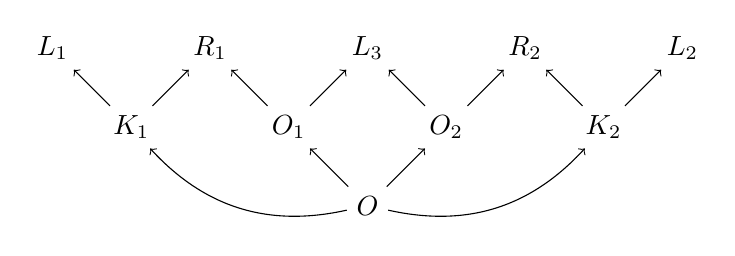
\begin{tikzpicture} %[scale=0.8]
      \node (o) at (0,-1) {\(O\)};
      \node (r3) at (0,1) {\(L_3\)};
      \node (o1) at (-1,0) {\(O_1\)};
      \node (o2) at (1,0) {\(O_2\)};
      \node (r1) at (-2,1) {\(R_1\)};
      \node (r2) at (2,1) {\(R_2\)};
      \node (l1) at (-4,1) {\(L_1\)};
      \node (l2) at (4,1) {\(L_2\)};
      \node (k1) at (-3,0) {\(K_1\)};
      \node (k2) at (3,0) {\(K_2\)};
      \draw [->] (o) -- (o1);
      \draw [->] (o) -- (o2);
      \draw [->] (o1) -- (r3);
      \draw [->] (o2) -- (r3);
      \draw [->] (o1) -- (r1);
      \draw [->] (o2) -- (r2);
      \draw [->] (k1) -- (r1);
      \draw [->] (k2) -- (r2);
      \draw [->] (k1) -- (l1);
      \draw [->] (k2) -- (l2);
      \draw [->] (o) to [bend left] (k1);
      \draw [->] (o) to [bend right] (k2);
    \end{tikzpicture}
    \]
  \item[constraints on decorating negative meets]
    Let $e_1,e_2,e_3$ be three events in $s$ such that there exists $\spa_1:L_1\remb O_1\lemb L_3$ and $\spa_2:L_2\remb O_2\lemb L_3$ two spans with $e_1\redl{-}_{\spa_1} e_3$ and $e_2\redl{-}_{\spa_2} e_3$.
    Let $O_1\remb O\lemb O_2$ be the pullback of the span $O_1\lemb L_3 \remb O_2$. Then one of the following holds:
    \begin{itemize}
    \item either there exists the morphisms $O\emb K_1$ and $O\emb K_2$ that commute in the diagram below;
    \item or there exists the morphism $O\emb K_1$ but no morphism $O\emb K_2$ that commutes. Then there exists $\spa':L_2\remb O'\lemb L_1$, with $\spa\subseteq \spa'$ for which $e_2\redl{-}_{\spa'} e_1$; %and $e_1$,$e_2$ are pairs for positive and negative influence w.r.t. $L_1\remb O\lemb L_2$.
    \end{itemize}
   \[
    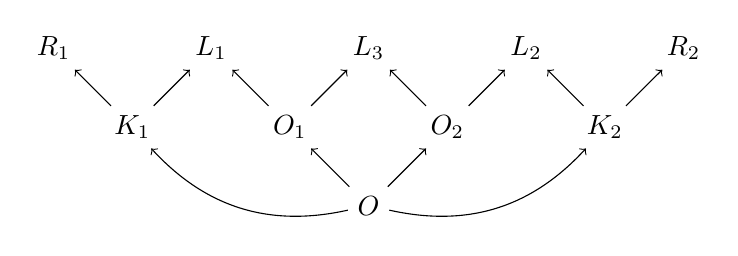
\begin{tikzpicture} %[scale=0.8]
      \node (o) at (0,-1) {\(O\)};
      \node (r3) at (0,1) {\(L_3\)};
      \node (o1) at (-1,0) {\(O_1\)};
      \node (o2) at (1,0) {\(O_2\)};
      \node (r1) at (-2,1) {\(L_1\)};
      \node (r2) at (2,1) {\(L_2\)};
      \node (l1) at (-4,1) {\(R_1\)};
      \node (l2) at (4,1) {\(R_2\)};
      \node (k1) at (-3,0) {\(K_1\)};
      \node (k2) at (3,0) {\(K_2\)};
      \draw [->] (o) -- (o1);
      \draw [->] (o) -- (o2);
      \draw [->] (o1) -- (r3);
      \draw [->] (o2) -- (r3);
      \draw [->] (o1) -- (r1);
      \draw [->] (o2) -- (r2);
      \draw [->] (k1) -- (r1);
      \draw [->] (k2) -- (r2);
      \draw [->] (k1) -- (l1);
      \draw [->] (k2) -- (l2);
      \draw [->] (o) to [bend left] (k1);
      \draw [->] (o) to [bend right] (k2);
    \end{tikzpicture}
    \]
    and $e_1$ and $e_2$ are pairs for positive and negative influence w.r.t. $L_1\remb O\lemb L_2$.
  \item[constraints on decorating positive forks]
    Let $e_1,e_2,e_3$ be three events in $s$ such that there exists $\spa_1:L_1\remb O_1\lemb R_3$ and $\spa_2:L_2\remb O_2\lemb R_3$ two spans with $e_3\redl{+}_{\spa_1} e_1$ and $e_3\redl{+}_{\spa_2} e_2$.
    Let $O_1\remb O\lemb O_2$ be the pullback of the span $O_1\lemb L_3 \remb O_2$. Then one of the following holds:
    \begin{itemize}
    \item either there exists the morphisms $O\emb K_1$ and $O\emb K_2$ that commute in the diagram below;
      %in which case $e_1$ and $e_2$ are pairs for positive and negative influence w.r.t. $L_1\remb O\lemb L_2$;
    \item or there exists the morphism $O\emb K_1$ but no morphism $O\emb K_2$ that commutes. Then there exists $\spa':L_2\remb O'\lemb L_1$, with $\spa\subseteq \spa'$ for which $e_2\redl{-}_{\spa'} e_1$;
      % and $e_1$ and $e_2$ are pairs for positive and negative influence w.r.t. $L_1\remb O\lemb L_2$.
    \end{itemize}
   \[
    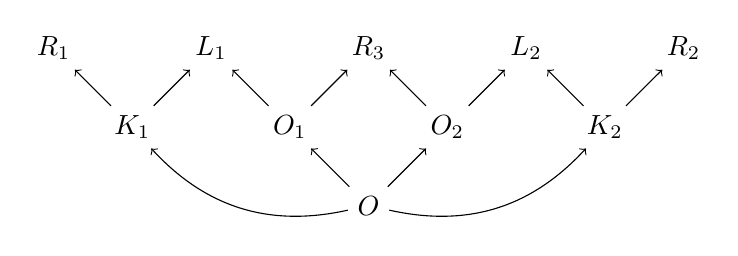
\begin{tikzpicture} %[scale=0.8]
      \node (o) at (0,-1) {\(O\)};
      \node (r3) at (0,1) {\(R_3\)};
      \node (o1) at (-1,0) {\(O_1\)};
      \node (o2) at (1,0) {\(O_2\)};
      \node (r1) at (-2,1) {\(L_1\)};
      \node (r2) at (2,1) {\(L_2\)};
      \node (l1) at (-4,1) {\(R_1\)};
      \node (l2) at (4,1) {\(R_2\)};
      \node (k1) at (-3,0) {\(K_1\)};
      \node (k2) at (3,0) {\(K_2\)};
      \draw [->] (o) -- (o1);
      \draw [->] (o) -- (o2);
      \draw [->] (o1) -- (r3);
      \draw [->] (o2) -- (r3);
      \draw [->] (o1) -- (r1);
      \draw [->] (o2) -- (r2);
      \draw [->] (k1) -- (r1);
      \draw [->] (k2) -- (r2);
      \draw [->] (k1) -- (l1);
      \draw [->] (k2) -- (l2);
      \draw [->] (o) to [bend left] (k1);
      \draw [->] (o) to [bend right] (k2);
    \end{tikzpicture}
    \]
    and $e_1$ and $e_2$ are pairs for positive and negative influence w.r.t. $L_1\remb O\lemb L_2$.
  \item[constraints on decorating negative forks]
    Let $e_1,e_2,e_3$ be three events in $s$ such that there exists $\spa_1:L_1\remb O_1\lemb R_3$ and $\spa_2:L_2\remb O_2\lemb R_3$ two spans with $e_3\redl{-}_{\spa_1} e_1$ and $e_3\redl{-}_{\spa_2} e_2$.
    Let $O_1\remb O\lemb O_2$ be the pullback of the span $O_1\lemb L_3 \remb O_2$. Then one of the following holds:
    \begin{itemize}
    \item either there exists the morphisms $O\emb K_1$ and $O\emb K_2$ that commute in the diagram below;
      %in which case $e_1$ and $e_2$ are pairs for positive and negative influence w.r.t. $L_1\remb O\lemb L_2$;
    \item or there exists the morphism $O\emb K_1$ but no morphism $O\emb K_2$ that commutes. Then there exists $\spa':L_2\remb O'\lemb L_1$, with $\spa\subseteq \spa'$ for which $e_2\redl{-}_{\spa'} e_1$;
      %and $e_1$ and $e_2$ are pairs for positive and negative influence w.r.t. $L_1\remb O\lemb L_2$.
    \end{itemize}
   \[
    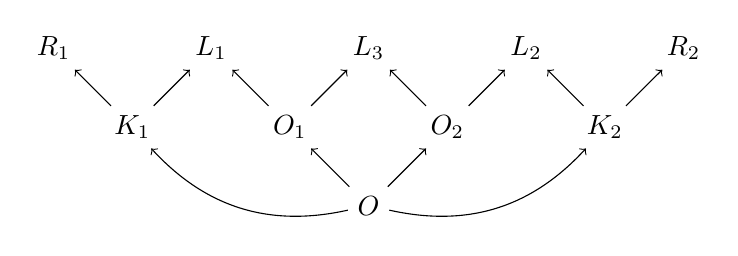
\begin{tikzpicture} %[scale=0.8]
      \node (o) at (0,-1) {\(O\)};
      \node (r3) at (0,1) {\(L_3\)};
      \node (o1) at (-1,0) {\(O_1\)};
      \node (o2) at (1,0) {\(O_2\)};
      \node (r1) at (-2,1) {\(L_1\)};
      \node (r2) at (2,1) {\(L_2\)};
      \node (l1) at (-4,1) {\(R_1\)};
      \node (l2) at (4,1) {\(R_2\)};
      \node (k1) at (-3,0) {\(K_1\)};
      \node (k2) at (3,0) {\(K_2\)};
      \draw [->] (o) -- (o1);
      \draw [->] (o) -- (o2);
      \draw [->] (o1) -- (r3);
      \draw [->] (o2) -- (r3);
      \draw [->] (o1) -- (r1);
      \draw [->] (o2) -- (r2);
      \draw [->] (k1) -- (r1);
      \draw [->] (k2) -- (r2);
      \draw [->] (k1) -- (l1);
      \draw [->] (k2) -- (l2);
      \draw [->] (o) to [bend left] (k1);
      \draw [->] (o) to [bend right] (k2);
    \end{tikzpicture}
    \]
    and $e_1$ and $e_2$ are pairs for positive and negative influence w.r.t. $L_1\remb O\lemb L_2$.
  \end{description}
  where $\labl(e_i)=r_i:L_i\remb K_i\lemb R_i$.
\end{definition}

\begin{lemma}
  \label{prop:constraints_poset}
  From a causal trace $\theta$ define the \emph{abstraction} function $\mathsf{decoration\_of\_trace}$ that maps a trace into a decorated poset as follows:
  \begin{align*}
    &\mathsf{decoration\_of\_trace}(t_i:M_i\overset{m,p}{\Rightarrow} M_{i+1}) = e_i \\
    &e_i \redl{+}_{\spa} e_j \iff t_i <_{\theta}^s t_j, \labl(t_i)\redl{+}_{\spa} \labl(t_j)\\
    &e_i \redl{-}_{\spa} e_j \iff t_i \dashv_{\theta} t_j, \labl(t_i) \redl{-}_{\spa} \labl(t_j).
  \end{align*}
  Then, for any causal trace $\theta$, $\mathsf{decoration\_of\_trace}(\theta)$ is a valid decorated poset.
\end{lemma}
The proof is in~\autoref{sec:valid_decor}.

In the following chain of abstractions:
  \[
  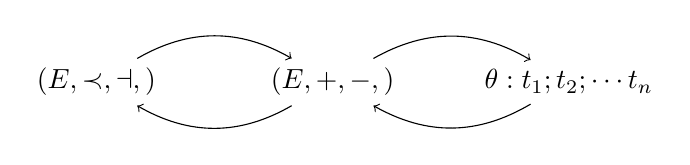
\begin{tikzpicture} %[scale=0.8]
%    \node (s) at (0,0) {\((E,\leq,\labl)\)};
    \node (as) at (3,0) {\((E,\prec,\dashv,\labl)\)};
    \node (ds) at (6,0) {\((E,\redl{+},\redl{-},\labl)\)};
    \node (trace) at (9,0) {\(\theta:t_1;t_2;\cdots t_n\)};
%    \draw [->] (s) to [bend left] (as);
%    \draw [->] (as) to [bend left] (s);
    \draw [->] (ds) to [bend left] (as);
    \draw [->] (as) to [bend left] (ds);
    \draw [->] (ds) to [bend left] (trace);
    \draw [->] (trace) to [bend left] (ds);
  \end{tikzpicture}
  \]
the definition above covers the abstractions from causal traces to decorated posets. The abstraction of~\autoref{def:abstraction} goes from causal traces to augmented posets. The concretisation function from an augmented poset to a decorated one returns all decorations of~\autoref{def:decorate_poset} that are valid.

%% \begin{example} - for the cover relation
%%   Let us consider the following rules:
%%   \begin{align*}
%%     r_1:\varepsilon \Rightarrow A, B\qquad r_2:A \Rightarrow C \qquad r_3: B,C \Rightarrow C
%%   \end{align*}
%%   and the trace
%%   \begin{align*}
%%     \varepsilon \overset{\emptyset,r_1}{\Rightarrow} A, B \overset{\id_A,r_2}{\Rightarrow} B,C \overset{id_{B,C},r_3}{\Rightarrow}C.
%%   \end{align*}
%%   Let us denote $t_1$, $t_2$ and $t_3$ the three transitions. We have that $t_1<t_3$, $t_2<t_3$ and $t_1< t_2$. If we "forget" that $t_1< t_3$ (as both $t_1<t_2$ and $t_2<t_3$ hold), we retrieve the following trace:
%%   \begin{align*}
%%     B_1 \overset{\emptyset,r_1}{\Rightarrow} B_1,A,B_2 \overset{\id_{A},r_2}{\Rightarrow} B_1,A,B_2,C \overset{id_{B_1,C},r_3}{\Rightarrow} B_2,A_1,C.
%%   \end{align*}
%% \end{example}

\begin{example}
  By abstracting the following trace $\theta=t_1;t_2;t_3$ we obtain a poset with three events $e_1,e_2,e_3$ such that $e_1\prec e_3$ and $e_2\prec e_3$:
  \[
  \theta:\varepsilon \Rightarrow A \Rightarrow A,A,B\Rightarrow A,A,B,C\qquad r_1: \varepsilon \Rightarrow A\qquad r_2: \varepsilon\Rightarrow A,B\qquad r_3: A,B\Rightarrow A,B,C
  \]
  We can come up with two decorations for such poset, where one of them leads to a invalid decorated poset:
  \begin{align*}
  \text{good decoration: }e_1\redl{+}_A e_3; e_2\redl{+}_B e_3\qquad
  \text{bad decoration: }e_1\redl{+}_A e_3; e_2\redl{+}_A e_3
  \end{align*}
  The bad decoration does not satisfy the constraint of decorating positive meets.
\end{example}

\begin{example}
  Let $e_1,e_2,e_3,e_4$ be four events in a poset such that $e_3\prec e_1$, $e_3\prec e_2$ and with the following corresponding rules
  \[
  r_3: A \Rightarrow B-A-C\qquad r_1: B-A\Rightarrow B-A-D \qquad r_2: A-C\Rightarrow A-C-D\qquad r_4: B-A-C\Rightarrow \varepsilon.
  \]
  we have that $e_3\redl{+}_{A-B} r_1$ and $e_3\redl{+}_{A-C} e_1$. Moreover events $e_1$ and $e_2$ are pairs for the negative influence of $e_4$ due to the resource $A$. Therefore $e_4\redl{-}_{A-B} e_1 \iff e_4\redl{-}_{A-C} e_2$.
\end{example}

\begin{example}
  Let $e_1,e_2,e_3$ be three events in a poset with $e_3\prec e_1$ and $e_3\prec e_2$ and with the rules $\labl(e_3)=r_3$, $\labl(e_1)=\labl(e_2)=r_1$ where
  \[
  r_3: \varepsilon \Rightarrow A\qquad r_1: A\Rightarrow \varepsilon.
  \]
  There is only one decoration: $e_3\redl{-}_{A} e_1$ and $e_3\redl{-}_{A} e_2$, which is invalid. The constraint on decoration positive forks is not satisfied. The resource $A$ produced by $e_3$ can only be consumed once.
  If, however, $e_1$ and $e_2$ do not consume $A$ but preserve it:
  \[
  r_3: \varepsilon \Rightarrow A\qquad r_1: A\Rightarrow A,B
  \]
  then indeed there is a valid decoration $e_3\redl{-}_{A} e_1$ and $e_3\redl{-}_{A} e_2$.
\end{example}

\subsection{From posets to traces}
\label{sec:refinement}

\begin{definition}[Refinement of an event in a trace]
  Let $E$ be a set of events and let $\theta$ be a trace. A refinement function is a bijection between events and transitions such that
  \[
  \mathtt{Ref}(e) = M\overset{m,\labl(e)}{\Rightarrow}N
  \]
  We say that $\mathtt{Ref}(e)$ is the refinement of $e$ in $\theta$ given a bijection $\mathtt{Ref}$.
\end{definition}

\begin{definition}[Concretisation of an augmented poset]
  \label{def:concret}
  Let $\underline s=(E,\cover,\prec,\dashv,\labl)$ be an augmented poset $s$.
  A \emph{concretisation} of $s$ is a triple $(s,\theta,\mathtt{Ref}:E\leftrightarrow\theta)$ such that $\mathtt{Ref}$ is a refinement function and such that
  \begin{align*}
    %e_1\cover e_2 \iff& \mathtt{Ref}(e_1) <_{\theta}\mathtt{Ref}(e_2)\\
    e_1\prec e_2 \iff& \mathtt{Ref}(e_1) \prec_{\theta}\mathtt{Ref}(e_2)\\
    e_1\dashv e_2 \iff& \mathtt{Ref}(e_1) \dashv_{\theta}\mathtt{Ref}(e_2)
  \end{align*}
  Define $\gamma(s)$ to be the set of all concretisations of $s$:
  \begin{align*}
    \gamma(s) = \{\theta: (s,\theta,\mathtt{Ref})\text{ is a concretisation of }s\}.
  \end{align*}
\end{definition}

\begin{theorem}
  Let $\theta$ be a causal trace. Then $\theta\subseteq\gamma(\alpha(\theta))$.
\end{theorem}
\begin{proof}
  Suffices to show that for any causal trace $\theta$ there exists a refinement bijection between $\alpha(\theta)$ and $\theta$ that satisfies the constraints in~\autoref{def:concret}. It follows from~\autoref{def:abstraction}.
\end{proof}

%%%%%the algorithm%%%%%%%

\begin{definition}[Linear extensions of posets]
  \label{def:linears}
  A linear extension of a poset $s=(E,\tleq)$ is any total order that extends the partial order $\tleq$. We denote $\linear(s)$ the set of all possible linear extensions of $s$. A linear extension of a augmented poset $s=(E,\cover,\prec,\dashv)$ is any total order such that
  \begin{align*}
    (E,\seq)\in\linear(s) \iff \forall e_1,e_2\in E, &e_1\leq e_2\implies e_1\seq e_2\\
    & e_1\dashv e_2\implies e_2\seq e_1.
  \end{align*}
\end{definition}
Note that linearisations do not create cycles, as follows from the definition of augmented posets.

\paragraph{A candidate for the concretisation}
Let $s = (E,\seq,\cover,\prec,\dashv,\labl)$ be a linear extension of an augmented poset. The function $\mathsf{concretise}(s,\emptyset,\emptyset)$ defined below returns a set of concretisations for $s$.
\begin{align*}
  &\mathsf{concretise}(s,s_1,\mathit{concretisations}_1) = \\
  &\quad\text{if }(E_s\setminus E_{s_1} = \emptyset)\text{ then return }\mathit{concretisations}_1\\
  &\quad e = \text{min}_{\sqsubset}(E_s\setminus E_{s_1})\\
  &\quad\mathit{concretisations}_2 = \emptyset \\
  &\quad\text{for each }(s_1^{\star},\theta_1,\mathtt{Ref}_1)\text{ in }\mathit{concretisations}_1\\
  &\quad\qquad s_2 = s\setminus\{s_1\cup\{e\}\}\\
  &\quad\qquad\text{for each }s_2^{\star}\text{ in }\mathsf{decorate}(s_2)\\
  %&\quad\qquad\qquad (s_1)^{\star} = \mathsf{decoration\_of\_trace}(\theta_1)\\
  &\quad\qquad\qquad \text{ if }s_2^{\star}\subseteq s_1^{\star}\text{ and }\mathsf{valid}(s_2^{\star})\text{ then }\\
  &\quad\qquad\qquad\qquad (\mathit{\theta_2},\mathtt{Ref}_2) = \mathsf{refine}(\theta_1,\mathtt{Ref}_1,s_2^{\star})\\
  &\quad\qquad\qquad\qquad \mathit{concretisations}_2 = \mathit{concretisations}_2 \cup (s_2^{\star},\mathit{\theta_2},\mathtt{Ref}_2)\\
  &\quad\text{return }\mathit{concretisations}_2
\end{align*}
where $\mathsf{decorate}$ returns a decoration of $s$ as in~\autoref{def:decorate_poset}, $\mathsf{decoration\_of\_trace}$ is an abstraction of a trace to its decorated poset, defined in the~\autoref{prop:constraints_poset}, $\mathsf{valid}$ is from~\autoref{def:constraints_poset} and lastly, $\mathsf{refine}$ is a function that extends a trace and a refinement to the new event $e$. We provide more details for $\mathsf{refine}$ in the appendix. Also in the appendix, we show that at each call of $\mathsf{concretise}$, the concretisations obtained so far are correct w.r.t.~\autoref{def:concret}.

\subsection{Interpreting inhibition on posets}
\label{sec:inhibition}

\begin{definition}[Refinement based on negative influence]
  \label{def:ref_neg_infl}
  Let $s_1,s_2$ be two augmented posets and let $(s_1,\theta_1,\mathtt{Ref}_1)$ and $(s_2,\theta_2,\mathtt{Ref}_2)$ be two concretisations for $s_1$ and $s_2$ respectively.
  Define $\mathtt{Ref}(e_1\in s_1\redl{-} e_2\in s_2)$ as the set of graphs $M$ for which the diagram below commutes:
  \[
  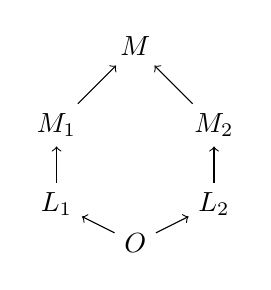
\begin{tikzpicture} %[scale=0.8]
    \node (o) at (0,-0.5) {\(O\)};
    \node (n) at (0,2) {\(M\)};
    \node (l1) at (-1,0) {\(L_1\)};
    \node (l2) at (1,0) {\(L_2\)};
    \node (n1) at (-1,1) {\(M_1\)};
    \node (n2) at (1,1) {\(M_2\)};
    \draw [->] (l1) -- (n1);
    \draw [->] (l2) -- (n2);
    \draw [->] (o) -- (l1);
    \draw [->] (o) -- (l2);
    \draw [->] (n1) -- (n);
    \draw [->] (n2) -- (n);
  \end{tikzpicture}
  \]
  where $\mathtt{Ref}_1(e_1) = M_1\Rightarrow N_1$, $\mathtt{Ref}_2(e_2) = M_2\Rightarrow N_2$, and $\labl(e_1)\redl{-}_{\spa}\labl(e_2)$, for some cospan $\spa:L_1\remb O\lemb L_2$.
\end{definition}
